% Options for packages loaded elsewhere
\PassOptionsToPackage{unicode}{hyperref}
\PassOptionsToPackage{hyphens}{url}
\PassOptionsToPackage{dvipsnames,svgnames,x11names}{xcolor}
%
\documentclass[
  letterpaper,
  DIV=11,
  numbers=noendperiod]{scrreprt}

\usepackage{amsmath,amssymb}
\usepackage{iftex}
\ifPDFTeX
  \usepackage[T1]{fontenc}
  \usepackage[utf8]{inputenc}
  \usepackage{textcomp} % provide euro and other symbols
\else % if luatex or xetex
  \usepackage{unicode-math}
  \defaultfontfeatures{Scale=MatchLowercase}
  \defaultfontfeatures[\rmfamily]{Ligatures=TeX,Scale=1}
\fi
\usepackage{lmodern}
\ifPDFTeX\else  
    % xetex/luatex font selection
\fi
% Use upquote if available, for straight quotes in verbatim environments
\IfFileExists{upquote.sty}{\usepackage{upquote}}{}
\IfFileExists{microtype.sty}{% use microtype if available
  \usepackage[]{microtype}
  \UseMicrotypeSet[protrusion]{basicmath} % disable protrusion for tt fonts
}{}
\makeatletter
\@ifundefined{KOMAClassName}{% if non-KOMA class
  \IfFileExists{parskip.sty}{%
    \usepackage{parskip}
  }{% else
    \setlength{\parindent}{0pt}
    \setlength{\parskip}{6pt plus 2pt minus 1pt}}
}{% if KOMA class
  \KOMAoptions{parskip=half}}
\makeatother
\usepackage{xcolor}
\setlength{\emergencystretch}{3em} % prevent overfull lines
\setcounter{secnumdepth}{5}
% Make \paragraph and \subparagraph free-standing
\ifx\paragraph\undefined\else
  \let\oldparagraph\paragraph
  \renewcommand{\paragraph}[1]{\oldparagraph{#1}\mbox{}}
\fi
\ifx\subparagraph\undefined\else
  \let\oldsubparagraph\subparagraph
  \renewcommand{\subparagraph}[1]{\oldsubparagraph{#1}\mbox{}}
\fi

\usepackage{color}
\usepackage{fancyvrb}
\newcommand{\VerbBar}{|}
\newcommand{\VERB}{\Verb[commandchars=\\\{\}]}
\DefineVerbatimEnvironment{Highlighting}{Verbatim}{commandchars=\\\{\}}
% Add ',fontsize=\small' for more characters per line
\usepackage{framed}
\definecolor{shadecolor}{RGB}{241,243,245}
\newenvironment{Shaded}{\begin{snugshade}}{\end{snugshade}}
\newcommand{\AlertTok}[1]{\textcolor[rgb]{0.68,0.00,0.00}{#1}}
\newcommand{\AnnotationTok}[1]{\textcolor[rgb]{0.37,0.37,0.37}{#1}}
\newcommand{\AttributeTok}[1]{\textcolor[rgb]{0.40,0.45,0.13}{#1}}
\newcommand{\BaseNTok}[1]{\textcolor[rgb]{0.68,0.00,0.00}{#1}}
\newcommand{\BuiltInTok}[1]{\textcolor[rgb]{0.00,0.23,0.31}{#1}}
\newcommand{\CharTok}[1]{\textcolor[rgb]{0.13,0.47,0.30}{#1}}
\newcommand{\CommentTok}[1]{\textcolor[rgb]{0.37,0.37,0.37}{#1}}
\newcommand{\CommentVarTok}[1]{\textcolor[rgb]{0.37,0.37,0.37}{\textit{#1}}}
\newcommand{\ConstantTok}[1]{\textcolor[rgb]{0.56,0.35,0.01}{#1}}
\newcommand{\ControlFlowTok}[1]{\textcolor[rgb]{0.00,0.23,0.31}{#1}}
\newcommand{\DataTypeTok}[1]{\textcolor[rgb]{0.68,0.00,0.00}{#1}}
\newcommand{\DecValTok}[1]{\textcolor[rgb]{0.68,0.00,0.00}{#1}}
\newcommand{\DocumentationTok}[1]{\textcolor[rgb]{0.37,0.37,0.37}{\textit{#1}}}
\newcommand{\ErrorTok}[1]{\textcolor[rgb]{0.68,0.00,0.00}{#1}}
\newcommand{\ExtensionTok}[1]{\textcolor[rgb]{0.00,0.23,0.31}{#1}}
\newcommand{\FloatTok}[1]{\textcolor[rgb]{0.68,0.00,0.00}{#1}}
\newcommand{\FunctionTok}[1]{\textcolor[rgb]{0.28,0.35,0.67}{#1}}
\newcommand{\ImportTok}[1]{\textcolor[rgb]{0.00,0.46,0.62}{#1}}
\newcommand{\InformationTok}[1]{\textcolor[rgb]{0.37,0.37,0.37}{#1}}
\newcommand{\KeywordTok}[1]{\textcolor[rgb]{0.00,0.23,0.31}{#1}}
\newcommand{\NormalTok}[1]{\textcolor[rgb]{0.00,0.23,0.31}{#1}}
\newcommand{\OperatorTok}[1]{\textcolor[rgb]{0.37,0.37,0.37}{#1}}
\newcommand{\OtherTok}[1]{\textcolor[rgb]{0.00,0.23,0.31}{#1}}
\newcommand{\PreprocessorTok}[1]{\textcolor[rgb]{0.68,0.00,0.00}{#1}}
\newcommand{\RegionMarkerTok}[1]{\textcolor[rgb]{0.00,0.23,0.31}{#1}}
\newcommand{\SpecialCharTok}[1]{\textcolor[rgb]{0.37,0.37,0.37}{#1}}
\newcommand{\SpecialStringTok}[1]{\textcolor[rgb]{0.13,0.47,0.30}{#1}}
\newcommand{\StringTok}[1]{\textcolor[rgb]{0.13,0.47,0.30}{#1}}
\newcommand{\VariableTok}[1]{\textcolor[rgb]{0.07,0.07,0.07}{#1}}
\newcommand{\VerbatimStringTok}[1]{\textcolor[rgb]{0.13,0.47,0.30}{#1}}
\newcommand{\WarningTok}[1]{\textcolor[rgb]{0.37,0.37,0.37}{\textit{#1}}}

\providecommand{\tightlist}{%
  \setlength{\itemsep}{0pt}\setlength{\parskip}{0pt}}\usepackage{longtable,booktabs,array}
\usepackage{calc} % for calculating minipage widths
% Correct order of tables after \paragraph or \subparagraph
\usepackage{etoolbox}
\makeatletter
\patchcmd\longtable{\par}{\if@noskipsec\mbox{}\fi\par}{}{}
\makeatother
% Allow footnotes in longtable head/foot
\IfFileExists{footnotehyper.sty}{\usepackage{footnotehyper}}{\usepackage{footnote}}
\makesavenoteenv{longtable}
\usepackage{graphicx}
\makeatletter
\def\maxwidth{\ifdim\Gin@nat@width>\linewidth\linewidth\else\Gin@nat@width\fi}
\def\maxheight{\ifdim\Gin@nat@height>\textheight\textheight\else\Gin@nat@height\fi}
\makeatother
% Scale images if necessary, so that they will not overflow the page
% margins by default, and it is still possible to overwrite the defaults
% using explicit options in \includegraphics[width, height, ...]{}
\setkeys{Gin}{width=\maxwidth,height=\maxheight,keepaspectratio}
% Set default figure placement to htbp
\makeatletter
\def\fps@figure{htbp}
\makeatother
\newlength{\cslhangindent}
\setlength{\cslhangindent}{1.5em}
\newlength{\csllabelwidth}
\setlength{\csllabelwidth}{3em}
\newlength{\cslentryspacingunit} % times entry-spacing
\setlength{\cslentryspacingunit}{\parskip}
\newenvironment{CSLReferences}[2] % #1 hanging-ident, #2 entry spacing
 {% don't indent paragraphs
  \setlength{\parindent}{0pt}
  % turn on hanging indent if param 1 is 1
  \ifodd #1
  \let\oldpar\par
  \def\par{\hangindent=\cslhangindent\oldpar}
  \fi
  % set entry spacing
  \setlength{\parskip}{#2\cslentryspacingunit}
 }%
 {}
\usepackage{calc}
\newcommand{\CSLBlock}[1]{#1\hfill\break}
\newcommand{\CSLLeftMargin}[1]{\parbox[t]{\csllabelwidth}{#1}}
\newcommand{\CSLRightInline}[1]{\parbox[t]{\linewidth - \csllabelwidth}{#1}\break}
\newcommand{\CSLIndent}[1]{\hspace{\cslhangindent}#1}

\KOMAoption{captions}{tableheading}
\makeatletter
\@ifpackageloaded{tcolorbox}{}{\usepackage[skins,breakable]{tcolorbox}}
\@ifpackageloaded{fontawesome5}{}{\usepackage{fontawesome5}}
\definecolor{quarto-callout-color}{HTML}{909090}
\definecolor{quarto-callout-note-color}{HTML}{0758E5}
\definecolor{quarto-callout-important-color}{HTML}{CC1914}
\definecolor{quarto-callout-warning-color}{HTML}{EB9113}
\definecolor{quarto-callout-tip-color}{HTML}{00A047}
\definecolor{quarto-callout-caution-color}{HTML}{FC5300}
\definecolor{quarto-callout-color-frame}{HTML}{acacac}
\definecolor{quarto-callout-note-color-frame}{HTML}{4582ec}
\definecolor{quarto-callout-important-color-frame}{HTML}{d9534f}
\definecolor{quarto-callout-warning-color-frame}{HTML}{f0ad4e}
\definecolor{quarto-callout-tip-color-frame}{HTML}{02b875}
\definecolor{quarto-callout-caution-color-frame}{HTML}{fd7e14}
\makeatother
\makeatletter
\makeatother
\makeatletter
\@ifpackageloaded{bookmark}{}{\usepackage{bookmark}}
\makeatother
\makeatletter
\@ifpackageloaded{caption}{}{\usepackage{caption}}
\AtBeginDocument{%
\ifdefined\contentsname
  \renewcommand*\contentsname{Table of contents}
\else
  \newcommand\contentsname{Table of contents}
\fi
\ifdefined\listfigurename
  \renewcommand*\listfigurename{List of Figures}
\else
  \newcommand\listfigurename{List of Figures}
\fi
\ifdefined\listtablename
  \renewcommand*\listtablename{List of Tables}
\else
  \newcommand\listtablename{List of Tables}
\fi
\ifdefined\figurename
  \renewcommand*\figurename{Figure}
\else
  \newcommand\figurename{Figure}
\fi
\ifdefined\tablename
  \renewcommand*\tablename{Table}
\else
  \newcommand\tablename{Table}
\fi
}
\@ifpackageloaded{float}{}{\usepackage{float}}
\floatstyle{ruled}
\@ifundefined{c@chapter}{\newfloat{codelisting}{h}{lop}}{\newfloat{codelisting}{h}{lop}[chapter]}
\floatname{codelisting}{Listing}
\newcommand*\listoflistings{\listof{codelisting}{List of Listings}}
\makeatother
\makeatletter
\@ifpackageloaded{caption}{}{\usepackage{caption}}
\@ifpackageloaded{subcaption}{}{\usepackage{subcaption}}
\makeatother
\makeatletter
\@ifpackageloaded{tcolorbox}{}{\usepackage[skins,breakable]{tcolorbox}}
\makeatother
\makeatletter
\@ifundefined{shadecolor}{\definecolor{shadecolor}{rgb}{.97, .97, .97}}
\makeatother
\makeatletter
\makeatother
\makeatletter
\makeatother
\ifLuaTeX
  \usepackage{selnolig}  % disable illegal ligatures
\fi
\IfFileExists{bookmark.sty}{\usepackage{bookmark}}{\usepackage{hyperref}}
\IfFileExists{xurl.sty}{\usepackage{xurl}}{} % add URL line breaks if available
\urlstyle{same} % disable monospaced font for URLs
\hypersetup{
  pdftitle={Global Families Project},
  pdfauthor={Global Families Project Team},
  colorlinks=true,
  linkcolor={blue},
  filecolor={Maroon},
  citecolor={Blue},
  urlcolor={Blue},
  pdfcreator={LaTeX via pandoc}}

\title{Global Families Project}
\author{Global Families Project Team}
\date{2023-06-22}

\begin{document}
\maketitle
\ifdefined\Shaded\renewenvironment{Shaded}{\begin{tcolorbox}[borderline west={3pt}{0pt}{shadecolor}, sharp corners, interior hidden, enhanced, frame hidden, breakable, boxrule=0pt]}{\end{tcolorbox}}\fi

\renewcommand*\contentsname{Table of contents}
{
\hypersetup{linkcolor=}
\setcounter{tocdepth}{2}
\tableofcontents
}
\bookmarksetup{startatroot}

\hypertarget{project-summary}{%
\chapter{Project Summary}\label{project-summary}}

Gender inequality perpetuates harmful norms that justify violence
against women and children and is associated with higher rates of family
violence.

Worldwide, parental physical abuse is a common form of family violence
that children are exposed to at alarming rates. Parental engagement in
physical abuse is linked to negative child outcomes including
depression, anxiety, and aggression that may persist into adulthood.
Globally, these continuing mental health and aggression problems may
have high financial costs, with effects both on social service systems
and developing economies.

Despite the substantial scholarship on parent- and family-level
predictors of parent-to-child physical violence, important questions
remain about societal-level predictors of parental physical abuse and
its associations with young children's development in developing and
transitional countries.

A further gap in prior literature is the lack of studies that have
examined potential moderators such as child age and household economic
status in the associations between gender inequality and parental
violence against children.

Using data from over 520,000 families in 57 low- and middle-income
countries (LMICs), the current project seeks to address these research
gaps by examining the associations of country-level gender inequality
and violent social contexts with caregivers' use of physically abusive
behavior and child social-emotional development. We will employ
multilevel models using data on parental physical violence against
children, family socio-economic characteristics, and children's
social-emotional development from the UNICEF Multiple Indicator Cluster
Surveys (MICS) and data on country-level gender inequality and violent
social contexts from the United Nations Development Programme on Human
Development and the World Health Organization Global Health Observatory.

The specific aims are to 1) examine the associations of gender
inequality with parental child physical abuse in LMICs, and the
moderating roles of child age and household economic status in these
associations, 2) examine the associations of violent social norms and
crimes with parental physical abuse in LMICs, and 3) examine the
associations of parental physical abuse with child social-emotional
development in the context of gender inequality and violent norms and
crimes in LMICs, and whether country-level normativeness of physical
abuse moderates these associations.

The proposed studies will advance the understanding of macro-level
social and economic indicators that perpetuate caregivers' physical
violence against children in international contexts. Study findings will
inform cross-cultural programs and policies that reduce gender
disparities and prevent parental physical abuse to promote child
social-emotional development across the globe.

In addition, these studies will provide rigorous research engagement
opportunities to undergraduate students and graduate students and
strengthen the research environment at the University of Michigan-Flint.

\bookmarksetup{startatroot}

\hypertarget{research-team}{%
\chapter{Research Team}\label{research-team}}

\textbf{Julie Ma, Principal Investigator}

Associate Professor of Social Work, UM-Flint

Professor Ma's research interests center around the effects of
neighborhood disadvantage and negative parenting on the well-being of
children. Her research builds on her experience in parent education
programs that serve families in marginalized communities in Michigan.
Much of her current research focuses on the risks of negative contextual
and family influences such as neighborhood poverty and disorganization,
and parental corporal punishment on behavior problems and maltreatment
in early childhood.

\textbf{Andy Grogan-Kaylor, Co-Investigator}

Sandra K. Danziger Collegiate Professor, Professor of Social Work

Professor Grogan-Kaylor's research focuses on knowledge development and
intervention research on children and families with the aim of reducing
violence against children and improving family and child wellbeing.
Grogan-Kaylor's current research projects examine parenting behaviors
such as physical punishment and parental expressions of emotional warmth
and support, and their effects on children's aggression, antisocial
behavior, anxiety, and depression.

\textbf{Shawna Lee, Co-Investigator}

Professor of Social Work

Professor Lee is a professor at the University of Michigan School of
Social Work. She is the director of the Parenting in Context Research
Lab and the director of the Program Evaluation Group at the School. Lee
has published on topics related to child maltreatment, fathers'
parenting, father-child relationships, parenting stress and family
functioning, and parental discipline. Her recent research focuses on
parenting and stress during the COVID-19 pandemic.

\bookmarksetup{startatroot}

\hypertarget{simulated-multi-country-data}{%
\chapter{Simulated Multi-Country
Data}\label{simulated-multi-country-data}}

This website makes use of simulated data. Data come from 30 hypothetical
countries. Data contain measures of a few key aspects of
parenting\footnote{We use the term parenting throughout this site, but
  are aware that such parenting may come from biological parents, or
  from other caregivers.} or caregiving that have proven salient in the
empirical literature on parenting to date. The outcome is
\texttt{aggression} against other children.

\begin{tcolorbox}[enhanced jigsaw, breakable, colback=white, leftrule=.75mm, coltitle=black, toprule=.15mm, arc=.35mm, colframe=quarto-callout-note-color-frame, colbacktitle=quarto-callout-note-color!10!white, left=2mm, title=\textcolor{quarto-callout-note-color}{\faInfo}\hspace{0.5em}{Download The Data}, rightrule=.15mm, toptitle=1mm, opacityback=0, opacitybacktitle=0.6, bottomrule=.15mm, bottomtitle=1mm, titlerule=0mm]

\begin{itemize}
\tightlist
\item
  \href{https://github.com/agrogan1/globalfamilies/raw/main/simulate-data/MICSsimulated.RData}{R
  format}
\item
  \href{https://github.com/agrogan1/globalfamilies/raw/main/simulate-data/MICSsimulated.dta}{Stata
  Format}
\item
  \href{https://github.com/agrogan1/globalfamilies/raw/main/simulate-data/MICSsimulated.sav}{SPSS}
\end{itemize}

\end{tcolorbox}

\begin{Shaded}
\begin{Highlighting}[]
\FunctionTok{load}\NormalTok{(}\StringTok{"./simulate{-}data/MICSsimulated.RData"}\NormalTok{)}
\end{Highlighting}
\end{Shaded}

\hypertarget{variables-and-variable-labels}{%
\section{Variables and Variable
Labels}\label{variables-and-variable-labels}}

\begin{Shaded}
\begin{Highlighting}[]
\NormalTok{pander}\SpecialCharTok{::}\FunctionTok{pander}\NormalTok{(labelled}\SpecialCharTok{::}\FunctionTok{look\_for}\NormalTok{(MICSsimulated)[}\DecValTok{1}\SpecialCharTok{:}\DecValTok{5}\NormalTok{])}
\end{Highlighting}
\end{Shaded}

\begin{longtable}[]{@{}
  >{\centering\arraybackslash}p{(\columnwidth - 8\tabcolsep) * \real{0.0833}}
  >{\centering\arraybackslash}p{(\columnwidth - 8\tabcolsep) * \real{0.1806}}
  >{\centering\arraybackslash}p{(\columnwidth - 8\tabcolsep) * \real{0.3611}}
  >{\centering\arraybackslash}p{(\columnwidth - 8\tabcolsep) * \real{0.1528}}
  >{\centering\arraybackslash}p{(\columnwidth - 8\tabcolsep) * \real{0.1528}}@{}}
\toprule\noalign{}
\begin{minipage}[b]{\linewidth}\centering
pos
\end{minipage} & \begin{minipage}[b]{\linewidth}\centering
variable
\end{minipage} & \begin{minipage}[b]{\linewidth}\centering
label
\end{minipage} & \begin{minipage}[b]{\linewidth}\centering
col\_type
\end{minipage} & \begin{minipage}[b]{\linewidth}\centering
missing
\end{minipage} \\
\midrule\noalign{}
\endhead
\bottomrule\noalign{}
\endlastfoot
1 & id & id & int & 0 \\
2 & country & country & int & 0 \\
3 & GII & gender inequality index & int & 0 \\
4 & cd1 & spank & int & 0 \\
5 & cd2 & beat & int & 0 \\
6 & cd3 & shout & int & 0 \\
7 & cd4 & explain & int & 0 \\
8 & aggression & aggression & int & 0 \\
\end{longtable}

\hypertarget{a-sample-of-the-data}{%
\section{A Sample Of The Data}\label{a-sample-of-the-data}}

A sample of the data is given below.

\begin{Shaded}
\begin{Highlighting}[]
\NormalTok{pander}\SpecialCharTok{::}\FunctionTok{pander}\NormalTok{(}\FunctionTok{head}\NormalTok{(MICSsimulated))}
\end{Highlighting}
\end{Shaded}

\hypertarget{tbl-simulateddata}{}
\begin{longtable}[]{@{}
  >{\centering\arraybackslash}p{(\columnwidth - 14\tabcolsep) * \real{0.0694}}
  >{\centering\arraybackslash}p{(\columnwidth - 14\tabcolsep) * \real{0.1389}}
  >{\centering\arraybackslash}p{(\columnwidth - 14\tabcolsep) * \real{0.0833}}
  >{\centering\arraybackslash}p{(\columnwidth - 14\tabcolsep) * \real{0.0833}}
  >{\centering\arraybackslash}p{(\columnwidth - 14\tabcolsep) * \real{0.0833}}
  >{\centering\arraybackslash}p{(\columnwidth - 14\tabcolsep) * \real{0.0833}}
  >{\centering\arraybackslash}p{(\columnwidth - 14\tabcolsep) * \real{0.0833}}
  >{\centering\arraybackslash}p{(\columnwidth - 14\tabcolsep) * \real{0.1806}}@{}}
\caption{\label{tbl-simulateddata}Simulated Multicountry
Data}\tabularnewline
\toprule\noalign{}
\begin{minipage}[b]{\linewidth}\centering
id
\end{minipage} & \begin{minipage}[b]{\linewidth}\centering
country
\end{minipage} & \begin{minipage}[b]{\linewidth}\centering
GII
\end{minipage} & \begin{minipage}[b]{\linewidth}\centering
cd1
\end{minipage} & \begin{minipage}[b]{\linewidth}\centering
cd2
\end{minipage} & \begin{minipage}[b]{\linewidth}\centering
cd3
\end{minipage} & \begin{minipage}[b]{\linewidth}\centering
cd4
\end{minipage} & \begin{minipage}[b]{\linewidth}\centering
aggression
\end{minipage} \\
\midrule\noalign{}
\endfirsthead
\toprule\noalign{}
\begin{minipage}[b]{\linewidth}\centering
id
\end{minipage} & \begin{minipage}[b]{\linewidth}\centering
country
\end{minipage} & \begin{minipage}[b]{\linewidth}\centering
GII
\end{minipage} & \begin{minipage}[b]{\linewidth}\centering
cd1
\end{minipage} & \begin{minipage}[b]{\linewidth}\centering
cd2
\end{minipage} & \begin{minipage}[b]{\linewidth}\centering
cd3
\end{minipage} & \begin{minipage}[b]{\linewidth}\centering
cd4
\end{minipage} & \begin{minipage}[b]{\linewidth}\centering
aggression
\end{minipage} \\
\midrule\noalign{}
\endhead
\bottomrule\noalign{}
\endlastfoot
1 & 1 & 20 & 0 & 1 & 0 & 1 & 1 \\
2 & 1 & 20 & 0 & 0 & 1 & 0 & 1 \\
3 & 1 & 20 & 0 & 0 & 0 & 1 & 1 \\
4 & 1 & 20 & 1 & 1 & 0 & 1 & 1 \\
5 & 1 & 20 & 0 & 0 & 1 & 1 & 0 \\
6 & 1 & 20 & 1 & 0 & 0 & 1 & 1 \\
\end{longtable}

\bookmarksetup{startatroot}

\hypertarget{a-quick-introduction-to-r}{%
\chapter{A Quick Introduction to R}\label{a-quick-introduction-to-r}}

\hypertarget{why-use-r}{%
\section{Why Use R?}\label{why-use-r}}

R has a reputation for being difficult to learn, and a lot of that
reputation is deserved. However, it is possible to teach R in an
accessible way, and \textbf{a little bit of R can take you a long way}.

\href{https://www.r-project.org/}{R} is open source, and therefore free,
statistical software that is particularly good at obtaining, analyzing
and visualizing data.

R Commands are stored in a \emph{script} or \emph{code} file that
usually ends in .R, e.g.~\texttt{myscript.R}. The command file is
distinct from your actual data, stored in an .RData file,
e.g.~\texttt{mydata.RData}.

A great deal of data analysis and visualization involves the same core
set of steps.

Given the fact that we often want to apply the same core set of tasks to
new questions and new data, there are ways to overcome the steep
learning curve and learn a replicable set of commands that can be
applied to problem after problem. \textbf{The same 5 to 10 lines of R
code can often be tweaked over and over again for multiple projects.}

\[\text{have a question} \rightarrow \text{get data} \rightarrow \text{process and clean data} \rightarrow\]
\[\text{visualize data} \rightarrow \text{analyze data} \rightarrow \text{make conclusions}\]

\hypertarget{get-r}{%
\section{Get R}\label{get-r}}

\href{https://www.r-project.org/}{R} is available at
\url{https://www.r-project.org/}. R is a lot easier to run if you run it
from RStudio, \url{http://www.rstudio.com}.

\hypertarget{get-data}{%
\section{Get Data}\label{get-data}}

Data often comes from other types of data files like SPSS, Stata, or
Excel. Especially in beginning R programming, getting the data into R
can be the most complicated part of your program.

\begin{Shaded}
\begin{Highlighting}[]
\FunctionTok{load}\NormalTok{(}\StringTok{"./simulate{-}data/MICSsimulated.RData"}\NormalTok{) }\CommentTok{\# data in R format}
\end{Highlighting}
\end{Shaded}

If data are in other formats, slightly different code may be required.

\begin{Shaded}
\begin{Highlighting}[]
\FunctionTok{library}\NormalTok{(haven) }\CommentTok{\# library for importing data }
\NormalTok{mydata }\OtherTok{\textless{}{-}} \FunctionTok{read\_sav}\NormalTok{(}\StringTok{"the/path/to/mySPSSfile.sav"}\NormalTok{) }\CommentTok{\# SPSS}
\NormalTok{mydata }\OtherTok{\textless{}{-}} \FunctionTok{read\_dta}\NormalTok{(}\StringTok{"the/path/to/myStatafile.dta"}\NormalTok{) }\CommentTok{\# Stata}

\FunctionTok{library}\NormalTok{(readxl) }\CommentTok{\# library for importing Excel files}
\NormalTok{mydata }\OtherTok{\textless{}{-}} \FunctionTok{read\_excel}\NormalTok{(}\StringTok{"the/path/to/mySpreadsheet.xls"}\NormalTok{)}

\FunctionTok{save}\NormalTok{(mydata, }\AttributeTok{file =} \StringTok{"mydata.RData"}\NormalTok{) }\CommentTok{\# save in R format}
\end{Highlighting}
\end{Shaded}

\hypertarget{process-and-clean-data}{%
\section{Process and Clean Data}\label{process-and-clean-data}}

The \texttt{\$} sign is a kind of ``connector''. \texttt{mydata\$x}
means: ``The variable \texttt{x} in the dataset called
\texttt{mydata}''.

\begin{Shaded}
\begin{Highlighting}[]
\NormalTok{MICSsimulated}\SpecialCharTok{$}\NormalTok{cd1[MICSsimulated}\SpecialCharTok{$}\NormalTok{cd1 }\SpecialCharTok{==} \SpecialCharTok{{-}}\DecValTok{9}\NormalTok{] }\OtherTok{\textless{}{-}} \ConstantTok{NA} \CommentTok{\# missing ({-}9) to NA}
\end{Highlighting}
\end{Shaded}

R makes a strong distinction between \emph{continuous} \emph{numeric}
variables that measure scales like mental health or neighborhood safety,
and \emph{categorical} \emph{factor variables} that measure non-ordered
categories like religious identity or gender identity.

Many statistical and graphical procedures are designed to recognize and
work with different variable types. You often \emph{don't} need to use
all of the options.
e.g.~\texttt{mydata\$w\ \textless{}-\ factor(mydata\$z)} will often work
just fine. \textbf{Changing variables from factor to numeric, and vice
versa can sometimes be the simple solution that solves a lot of problems
when you are trying to graph your variables.}

\begin{Shaded}
\begin{Highlighting}[]
\NormalTok{MICSsimulated}\SpecialCharTok{$}\NormalTok{aggression }\OtherTok{\textless{}{-}} 
  \FunctionTok{factor}\NormalTok{(MICSsimulated}\SpecialCharTok{$}\NormalTok{aggression, }\CommentTok{\# original numeric variable}
         \AttributeTok{levels =} \FunctionTok{c}\NormalTok{(}\DecValTok{0}\NormalTok{, }\DecValTok{1}\NormalTok{), }
         \AttributeTok{labels =} \FunctionTok{c}\NormalTok{(}\StringTok{"no aggression"}\NormalTok{, }\StringTok{"aggression"}\NormalTok{), }
         \AttributeTok{ordered =} \ConstantTok{TRUE}\NormalTok{) }\CommentTok{\# whether order matters}

\CommentTok{\# MICSsimulated$z \textless{}{-} as.numeric(MICSsimulated$w) \# factor to numeric}
\end{Highlighting}
\end{Shaded}

\hypertarget{visualize-data}{%
\section{Visualize Data}\label{visualize-data}}

\hypertarget{histogram}{%
\subsection{Histogram}\label{histogram}}

\begin{Shaded}
\begin{Highlighting}[]
\FunctionTok{hist}\NormalTok{(MICSsimulated}\SpecialCharTok{$}\NormalTok{GII, }\CommentTok{\# what I\textquotesingle{}m graphing}
        \AttributeTok{main =} \StringTok{"Gender Inequality Index"}\NormalTok{, }\CommentTok{\# title}
        \AttributeTok{xlab =} \StringTok{"GII"}\NormalTok{, }\CommentTok{\# label for x axis}
        \AttributeTok{col =} \StringTok{"blue"}\NormalTok{) }\CommentTok{\# color}
\end{Highlighting}
\end{Shaded}

\begin{figure}[H]

{\centering 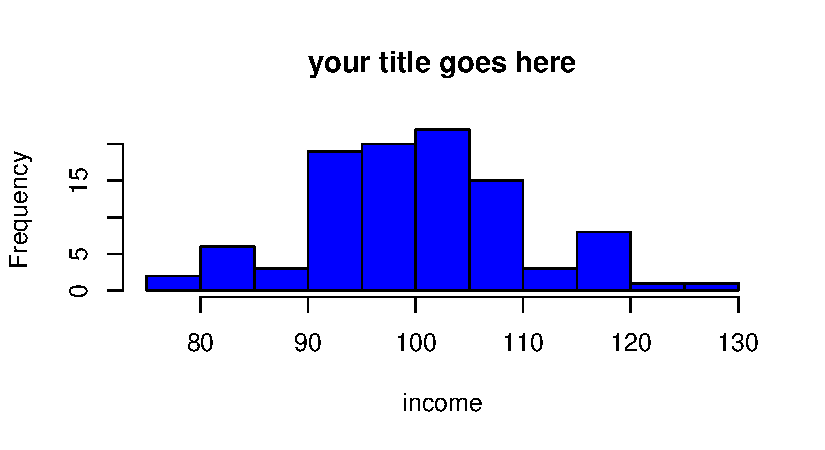
\includegraphics{quick-intro-R_files/figure-pdf/unnamed-chunk-5-1.pdf}

}

\end{figure}

\begin{tcolorbox}[enhanced jigsaw, breakable, colback=white, leftrule=.75mm, coltitle=black, toprule=.15mm, arc=.35mm, colframe=quarto-callout-tip-color-frame, colbacktitle=quarto-callout-tip-color!10!white, left=2mm, title=\textcolor{quarto-callout-tip-color}{\faLightbulb}\hspace{0.5em}{Tip}, rightrule=.15mm, toptitle=1mm, opacityback=0, opacitybacktitle=0.6, bottomrule=.15mm, bottomtitle=1mm, titlerule=0mm]

You often \emph{don't} need to use all of the options.
e.g.~\texttt{hist(mydata\$x)} will work just fine.

\end{tcolorbox}

\hypertarget{barplot}{%
\subsection{Barplot}\label{barplot}}

\begin{Shaded}
\begin{Highlighting}[]
\FunctionTok{barplot}\NormalTok{(}\FunctionTok{table}\NormalTok{(MICSsimulated}\SpecialCharTok{$}\NormalTok{aggression), }\CommentTok{\# what I\textquotesingle{}m graphing}
        \AttributeTok{main =} \StringTok{"Child Displays Aggression"}\NormalTok{, }\CommentTok{\# title}
        \AttributeTok{xlab =} \StringTok{"Aggression"}\NormalTok{, }\CommentTok{\# label for x axis}
        \AttributeTok{col =} \StringTok{"gold"}\NormalTok{) }\CommentTok{\# color}
\end{Highlighting}
\end{Shaded}

\begin{figure}[H]

{\centering 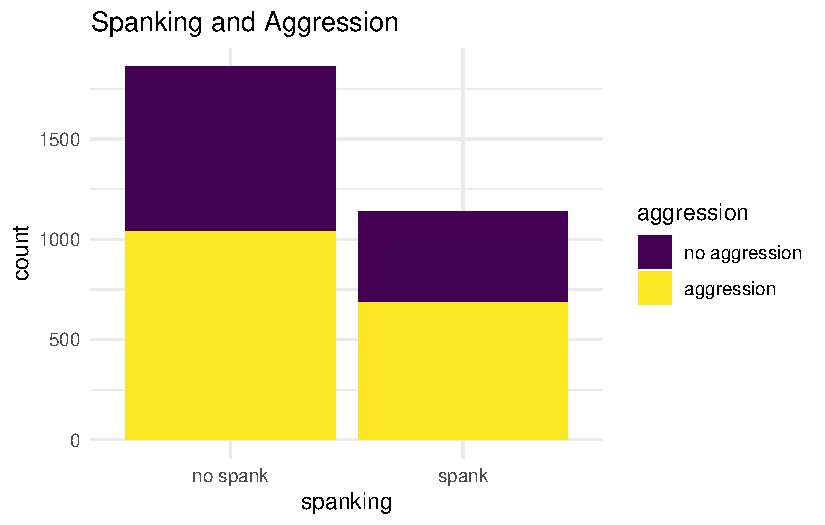
\includegraphics{quick-intro-R_files/figure-pdf/unnamed-chunk-6-1.pdf}

}

\end{figure}

\begin{tcolorbox}[enhanced jigsaw, breakable, colback=white, leftrule=.75mm, coltitle=black, toprule=.15mm, arc=.35mm, colframe=quarto-callout-tip-color-frame, colbacktitle=quarto-callout-tip-color!10!white, left=2mm, title=\textcolor{quarto-callout-tip-color}{\faLightbulb}\hspace{0.5em}{Tip}, rightrule=.15mm, toptitle=1mm, opacityback=0, opacitybacktitle=0.6, bottomrule=.15mm, bottomtitle=1mm, titlerule=0mm]

You often \emph{don't} need to use all of the options.
e.g.~\texttt{barplot(table(mydata\$z))} will work just fine.

\end{tcolorbox}

\hypertarget{analyze-data-descriptive-statistics}{%
\section{Analyze Data: Descriptive
Statistics}\label{analyze-data-descriptive-statistics}}

\begin{Shaded}
\begin{Highlighting}[]
\FunctionTok{summary}\NormalTok{(mydata}\SpecialCharTok{$}\NormalTok{x) }\CommentTok{\# for continuous or factor variables}

\FunctionTok{table}\NormalTok{(mydata}\SpecialCharTok{$}\NormalTok{z) }\CommentTok{\# especially suitable for factor variables}
\end{Highlighting}
\end{Shaded}

\begin{Shaded}
\begin{Highlighting}[]
\FunctionTok{summary}\NormalTok{(MICSsimulated}\SpecialCharTok{$}\NormalTok{GII)}
\end{Highlighting}
\end{Shaded}

\begin{verbatim}
   Min. 1st Qu.  Median    Mean 3rd Qu.    Max. 
   15.0    22.0    24.0    24.2    27.0    31.0 
\end{verbatim}

\begin{Shaded}
\begin{Highlighting}[]
\FunctionTok{table}\NormalTok{(MICSsimulated}\SpecialCharTok{$}\NormalTok{aggression)}
\end{Highlighting}
\end{Shaded}

\begin{verbatim}

no aggression    aggression 
         1274          1726 
\end{verbatim}

\bookmarksetup{startatroot}

\hypertarget{references}{%
\chapter*{References}\label{references}}
\addcontentsline{toc}{chapter}{References}

\markboth{References}{References}

\hypertarget{refs}{}
\begin{CSLReferences}{1}{0}
\leavevmode\vadjust pre{\hypertarget{ref-Kreft1998}{}}%
Kreft, I., \& de Leeuw, J. (1998). \emph{Introducing multilevel
modeling}. SAGE Publications.
\url{https://doi.org/10.4135/9781849209366}

\leavevmode\vadjust pre{\hypertarget{ref-Luke2004}{}}%
Luke, D. (2004). \emph{Multilevel modeling}. SAGE Publications, Inc.
\url{https://doi.org/10.4135/9781412985147}

\leavevmode\vadjust pre{\hypertarget{ref-RabeHesketh2022}{}}%
Rabe-Hesketh, S., \& Skrondal, A. (2022). Multilevel and longitudinal
modeling using {S}tata. In \emph{Stata Press} (4th ed.). Stata Press.

\leavevmode\vadjust pre{\hypertarget{ref-Raudenbush2002}{}}%
Raudenbush, S. W., \& Bryk, A. S. (2002). \emph{Hierarchical linear
models: Applications and data analysis methods} (pp. xxiv, 485 p.). Sage
Publications.

\leavevmode\vadjust pre{\hypertarget{ref-Singer2003}{}}%
Singer, J. D., \& Willett, J. B. (2003). Applied longitudinal data
analysis : Modeling change and event occurrence. In \emph{Applied
longitudinal data analysis : modeling change and event occurrence}.
Oxford University Press.

\end{CSLReferences}

\cleardoublepage
\phantomsection
\addcontentsline{toc}{part}{Appendices}
\appendix

\hypertarget{simulating-mics-data}{%
\chapter{Simulating MICS Data}\label{simulating-mics-data}}

This appendix details the process of creating the simulated MICS data
that is employed in the examples on this website.

MICS data are freely available, but usage of MICS requires completing a
user agreement, and registering for a user account, on the MICS website,
and thus MICS data should not be shared openly on a public website.

This Appendix is highly technical. It is not necessary to understand
this Appendix to benefit from the rest of this website. However, the
details of creating this simulated data may be of interest to some
users.

\hypertarget{call-relevant-libraries}{%
\section{Call Relevant Libraries}\label{call-relevant-libraries}}

We need to call a number of relevant R libraries to simulate the data.

\begin{Shaded}
\begin{Highlighting}[]
\FunctionTok{library}\NormalTok{(tibble) }\CommentTok{\# new dataframes}

\FunctionTok{library}\NormalTok{(ggplot2) }\CommentTok{\# nifty graphs}

\FunctionTok{library}\NormalTok{(labelled) }\CommentTok{\# labels}

\FunctionTok{library}\NormalTok{(haven) }\CommentTok{\# write Stata}

\FunctionTok{library}\NormalTok{(tidyr) }\CommentTok{\# tidy data}

\FunctionTok{library}\NormalTok{(dplyr) }\CommentTok{\# wrangle data}

\FunctionTok{library}\NormalTok{(lme4) }\CommentTok{\# multilevel models}

\FunctionTok{library}\NormalTok{(sjPlot) }\CommentTok{\# nice tables}
\end{Highlighting}
\end{Shaded}

\hypertarget{setup-some-basic-parameters-of-the-data}{%
\section{Setup Some Basic Parameters of the
Data}\label{setup-some-basic-parameters-of-the-data}}

Because simulation is a random process, we set a \emph{random seed} so
that the simulation produces the same data set each time it is run.

We are going to simulate data with 30 countries, and 100 individuals per
country.

\begin{Shaded}
\begin{Highlighting}[]
\FunctionTok{set.seed}\NormalTok{(}\DecValTok{1234}\NormalTok{) }\CommentTok{\# random seed}

\NormalTok{N\_countries }\OtherTok{\textless{}{-}} \DecValTok{30} \CommentTok{\# number of countries}

\NormalTok{N }\OtherTok{\textless{}{-}} \DecValTok{100} \CommentTok{\# sample size / country}
\end{Highlighting}
\end{Shaded}

\hypertarget{simulate-data-based-on-mics}{%
\section{Simulate Data Based on
MICS}\label{simulate-data-based-on-mics}}

This is multilevel data where individuals are nested, or clustered,
inside countries. Excellent technical and pedagogical discussions of
multilevel models can be found in Raudenbush \& Bryk (2002), Singer \&
Willett (2003), Rabe-Hesketh \& Skrondal (2022), Luke (2004), and Kreft
\& de Leeuw (1998).

\hypertarget{level-2}{%
\subsection{Level 2}\label{level-2}}

Simulating the second level of the data is relatively easy. We simply
need to provide the number of countries, and then generate random
effects for each country. Random effects are discussed in the above
references, but essentially represent country level differences in the
data.

We also create \texttt{GII}, a gender inequality index variable, since
this is a country level, or Level 2 variable.

\begin{Shaded}
\begin{Highlighting}[]
\NormalTok{country }\OtherTok{\textless{}{-}} \FunctionTok{seq}\NormalTok{(}\DecValTok{1}\SpecialCharTok{:}\NormalTok{N\_countries) }\CommentTok{\# sequence 1 to 30}

\NormalTok{GII }\OtherTok{\textless{}{-}} \FunctionTok{rbinom}\NormalTok{(N\_countries, }\DecValTok{100}\NormalTok{, .}\DecValTok{25}\NormalTok{) }\CommentTok{\# gender inequality index}

\NormalTok{u0 }\OtherTok{\textless{}{-}} \FunctionTok{rnorm}\NormalTok{(N\_countries, }\DecValTok{0}\NormalTok{, .}\DecValTok{25}\NormalTok{) }\CommentTok{\# random intercept}

\NormalTok{u1 }\OtherTok{\textless{}{-}} \FunctionTok{rnorm}\NormalTok{(N\_countries, }\DecValTok{0}\NormalTok{, .}\DecValTok{05}\NormalTok{) }\CommentTok{\# random slope}

\NormalTok{randomeffects }\OtherTok{\textless{}{-}} \FunctionTok{data.frame}\NormalTok{(country, GII, u0, u1) }\CommentTok{\# dataframe of random effects}
\end{Highlighting}
\end{Shaded}

\hypertarget{level-1}{%
\subsection{Level 1}\label{level-1}}

Simulating the Level 1 data is more complex.

We \texttt{uncount} the data by 100 to create 100 observations for each
country. We then create an \texttt{id} number.

We create randomly simulated parental discipline variables with
proportions similar to those in MICS.

Lastly, we need to create the dependent variable. Because this is a
dichotomous outcome, the process is somewhat complex. We need to craete
a linear combination \texttt{z}, using regression weights derived from
MICS. We then calculate predicted probabilities, and lastly generate a
dichotomous \texttt{aggression} outcome from those probabilities.

\begin{Shaded}
\begin{Highlighting}[]
\NormalTok{MICSsimulated }\OtherTok{\textless{}{-}}\NormalTok{ randomeffects }\SpecialCharTok{\%\textgreater{}\%} 
  \FunctionTok{uncount}\NormalTok{(N) }\SpecialCharTok{\%\textgreater{}\%} \CommentTok{\# N individuals / country}
  \FunctionTok{mutate}\NormalTok{(}\AttributeTok{id =} \FunctionTok{row\_number}\NormalTok{()) }\SpecialCharTok{\%\textgreater{}\%} \CommentTok{\# unique id}
  \FunctionTok{mutate}\NormalTok{(}\AttributeTok{cd1 =} \FunctionTok{rbinom}\NormalTok{(N }\SpecialCharTok{*}\NormalTok{ N\_countries, }\DecValTok{1}\NormalTok{, .}\DecValTok{38}\NormalTok{), }\CommentTok{\# spank}
         \AttributeTok{cd2 =} \FunctionTok{rbinom}\NormalTok{(N }\SpecialCharTok{*}\NormalTok{ N\_countries, }\DecValTok{1}\NormalTok{, .}\DecValTok{05}\NormalTok{), }\CommentTok{\# beat}
         \AttributeTok{cd3 =} \FunctionTok{rbinom}\NormalTok{(N }\SpecialCharTok{*}\NormalTok{ N\_countries, }\DecValTok{1}\NormalTok{, .}\DecValTok{64}\NormalTok{), }\CommentTok{\# shout}
         \AttributeTok{cd4 =} \FunctionTok{rbinom}\NormalTok{(N }\SpecialCharTok{*}\NormalTok{ N\_countries, }\DecValTok{1}\NormalTok{, .}\DecValTok{78}\NormalTok{)) }\SpecialCharTok{\%\textgreater{}\%} \CommentTok{\# explain}
  \FunctionTok{mutate}\NormalTok{(}\AttributeTok{z =} \DecValTok{0} \SpecialCharTok{+} \CommentTok{\# linear combination based on MICS}
\NormalTok{           .}\DecValTok{01} \SpecialCharTok{*}\NormalTok{ GII }\SpecialCharTok{+}
\NormalTok{           .}\DecValTok{23} \SpecialCharTok{*}\NormalTok{ cd1 }\SpecialCharTok{+}
\NormalTok{           .}\DecValTok{52} \SpecialCharTok{*}\NormalTok{ cd2 }\SpecialCharTok{+}
\NormalTok{           .}\DecValTok{42} \SpecialCharTok{*}\NormalTok{ cd3 }\SpecialCharTok{+}
           \SpecialCharTok{{-}}\NormalTok{.}\DecValTok{21} \SpecialCharTok{*}\NormalTok{ cd4 }\SpecialCharTok{+} 
\NormalTok{           u0) }\SpecialCharTok{\%\textgreater{}\%}
  \FunctionTok{mutate}\NormalTok{(}\AttributeTok{p =} \FunctionTok{exp}\NormalTok{(z) }\SpecialCharTok{/}\NormalTok{ (}\DecValTok{1} \SpecialCharTok{+} \FunctionTok{exp}\NormalTok{(z))) }\SpecialCharTok{\%\textgreater{}\%} \CommentTok{\# probability}
  \FunctionTok{mutate}\NormalTok{(}\AttributeTok{aggression =} \FunctionTok{rbinom}\NormalTok{(N }\SpecialCharTok{*}\NormalTok{ N\_countries, }\DecValTok{1}\NormalTok{, p)) }\SpecialCharTok{\%\textgreater{}\%} \CommentTok{\# binomial y}
  \FunctionTok{select}\NormalTok{(id, country, GII,}
\NormalTok{         cd1, cd2, cd3, cd4, }
\NormalTok{         aggression)}
\end{Highlighting}
\end{Shaded}

\hypertarget{variable-labels}{%
\subsection{Variable Labels}\label{variable-labels}}

We add variable labels to the data which will help us to understand the
data as we analyze it.

\begin{Shaded}
\begin{Highlighting}[]
\FunctionTok{var\_label}\NormalTok{(MICSsimulated}\SpecialCharTok{$}\NormalTok{id) }\OtherTok{\textless{}{-}} \StringTok{"id"}

\FunctionTok{var\_label}\NormalTok{(MICSsimulated}\SpecialCharTok{$}\NormalTok{country) }\OtherTok{\textless{}{-}} \StringTok{"country"}

\FunctionTok{var\_label}\NormalTok{(MICSsimulated}\SpecialCharTok{$}\NormalTok{GII) }\OtherTok{\textless{}{-}} \StringTok{"gender inequality index"}

\FunctionTok{var\_label}\NormalTok{(MICSsimulated}\SpecialCharTok{$}\NormalTok{cd1) }\OtherTok{\textless{}{-}} \StringTok{"spank"}

\FunctionTok{var\_label}\NormalTok{(MICSsimulated}\SpecialCharTok{$}\NormalTok{cd2) }\OtherTok{\textless{}{-}} \StringTok{"beat"}

\FunctionTok{var\_label}\NormalTok{(MICSsimulated}\SpecialCharTok{$}\NormalTok{cd3) }\OtherTok{\textless{}{-}} \StringTok{"shout"}

\FunctionTok{var\_label}\NormalTok{(MICSsimulated}\SpecialCharTok{$}\NormalTok{cd4) }\OtherTok{\textless{}{-}} \StringTok{"explain"}

\FunctionTok{var\_label}\NormalTok{(MICSsimulated}\SpecialCharTok{$}\NormalTok{aggression) }\OtherTok{\textless{}{-}} \StringTok{"aggression"}

\NormalTok{pander}\SpecialCharTok{::}\FunctionTok{pander}\NormalTok{(labelled}\SpecialCharTok{::}\FunctionTok{look\_for}\NormalTok{(MICSsimulated)[}\DecValTok{1}\SpecialCharTok{:}\DecValTok{5}\NormalTok{]) }\CommentTok{\# list out variable labels}
\end{Highlighting}
\end{Shaded}

\begin{longtable}[]{@{}
  >{\centering\arraybackslash}p{(\columnwidth - 8\tabcolsep) * \real{0.0833}}
  >{\centering\arraybackslash}p{(\columnwidth - 8\tabcolsep) * \real{0.1806}}
  >{\centering\arraybackslash}p{(\columnwidth - 8\tabcolsep) * \real{0.3611}}
  >{\centering\arraybackslash}p{(\columnwidth - 8\tabcolsep) * \real{0.1528}}
  >{\centering\arraybackslash}p{(\columnwidth - 8\tabcolsep) * \real{0.1528}}@{}}
\toprule\noalign{}
\begin{minipage}[b]{\linewidth}\centering
pos
\end{minipage} & \begin{minipage}[b]{\linewidth}\centering
variable
\end{minipage} & \begin{minipage}[b]{\linewidth}\centering
label
\end{minipage} & \begin{minipage}[b]{\linewidth}\centering
col\_type
\end{minipage} & \begin{minipage}[b]{\linewidth}\centering
missing
\end{minipage} \\
\midrule\noalign{}
\endhead
\bottomrule\noalign{}
\endlastfoot
1 & id & id & int & 0 \\
2 & country & country & int & 0 \\
3 & GII & gender inequality index & int & 0 \\
4 & cd1 & spank & int & 0 \\
5 & cd2 & beat & int & 0 \\
6 & cd3 & shout & int & 0 \\
7 & cd4 & explain & int & 0 \\
8 & aggression & aggression & int & 0 \\
\end{longtable}

\hypertarget{explore-the-simulated-data-with-a-graph}{%
\section{Explore The Simulated Data With A
Graph}\label{explore-the-simulated-data-with-a-graph}}

Exploring the simulated data with a graph helps us to ensure that we
have simulated plausible data.

\begin{Shaded}
\begin{Highlighting}[]
\FunctionTok{ggplot}\NormalTok{(MICSsimulated,}
       \FunctionTok{aes}\NormalTok{(}\AttributeTok{x =}\NormalTok{ cd1, }\CommentTok{\# x is spanking}
           \AttributeTok{y =}\NormalTok{ aggression, }\CommentTok{\# y is aggression}
           \AttributeTok{color =} \FunctionTok{factor}\NormalTok{(country))) }\SpecialCharTok{+} \CommentTok{\# color is country}
  \FunctionTok{geom\_smooth}\NormalTok{(}\AttributeTok{method =} \StringTok{"glm"}\NormalTok{, }\CommentTok{\# glm smoother}
              \AttributeTok{method.args =} \FunctionTok{list}\NormalTok{(}\AttributeTok{family =} \StringTok{"binomial"}\NormalTok{),}
              \AttributeTok{alpha =}\NormalTok{ .}\DecValTok{1}\NormalTok{) }\SpecialCharTok{+} \CommentTok{\# transparency for CI\textquotesingle{}s}
  \FunctionTok{labs}\NormalTok{(}\AttributeTok{title =} \StringTok{"Aggression as a Function of Spanking"}\NormalTok{,}
       \AttributeTok{x =} \StringTok{"spank"}\NormalTok{,}
       \AttributeTok{y =} \StringTok{"aggression"}\NormalTok{) }\SpecialCharTok{+}
  \FunctionTok{scale\_color\_viridis\_d}\NormalTok{(}\AttributeTok{name =} \StringTok{"Country"}\NormalTok{) }\SpecialCharTok{+} \CommentTok{\# nice colors}
  \FunctionTok{theme\_minimal}\NormalTok{()}
\end{Highlighting}
\end{Shaded}

\begin{figure}[H]

{\centering 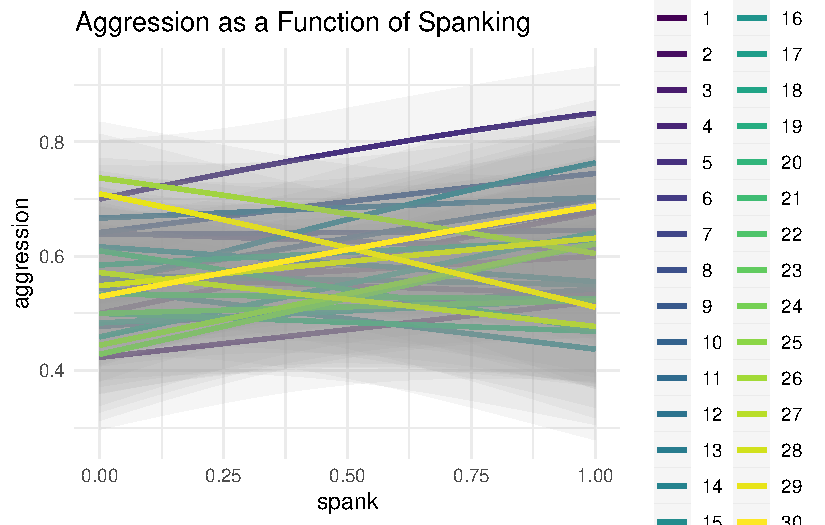
\includegraphics{simulate-data_files/figure-pdf/unnamed-chunk-6-1.pdf}

}

\end{figure}

\hypertarget{explore-the-simulated-data-with-a-logistic-regression}{%
\section{Explore The Simulated Data With A Logistic
Regression}\label{explore-the-simulated-data-with-a-logistic-regression}}

Similarly, exploring the data with a logistic regression confirms that
we have created plausible data.

\begin{Shaded}
\begin{Highlighting}[]
\NormalTok{fit1 }\OtherTok{\textless{}{-}} \FunctionTok{glmer}\NormalTok{(aggression }\SpecialCharTok{\textasciitilde{}}\NormalTok{ cd1 }\SpecialCharTok{+}\NormalTok{ cd2 }\SpecialCharTok{+}\NormalTok{ cd3 }\SpecialCharTok{+}\NormalTok{ cd4 }\SpecialCharTok{+}\NormalTok{ GII }\SpecialCharTok{+}
\NormalTok{                (}\DecValTok{1} \SpecialCharTok{|}\NormalTok{ country), }
              \AttributeTok{family =} \StringTok{"binomial"}\NormalTok{,}
              \AttributeTok{data =}\NormalTok{ MICSsimulated,}
              \AttributeTok{control =} \FunctionTok{glmerControl}\NormalTok{(}\AttributeTok{optimizer =}\StringTok{"bobyqa"}\NormalTok{))}

\FunctionTok{tab\_model}\NormalTok{(fit1, }\CommentTok{\# nice table}
          \AttributeTok{transform =} \ConstantTok{NULL}\NormalTok{) }\CommentTok{\# untransformed estimates}
\end{Highlighting}
\end{Shaded}

~

aggression

Predictors

Log-Odds

CI

p

(Intercept)

-0.42

-1.05~--~0.21

0.188

spank

0.16

0.01~--~0.32

\textbf{0.034}

beat

0.61

0.25~--~0.96

\textbf{0.001}

shout

0.35

0.20~--~0.51

\textbf{\textless0.001}

explain

-0.41

-0.59~--~-0.23

\textbf{\textless0.001}

gender inequality index

0.03

0.01~--~0.05

\textbf{0.015}

Random Effects

σ\textsuperscript{2}

3.29

τ\textsubscript{00} \textsubscript{country}

0.03

ICC

0.01

N \textsubscript{country}

30

Observations

3000

Marginal R\textsuperscript{2} / Conditional R\textsuperscript{2}

0.029 / 0.037

\hypertarget{write-data-to-various-formats}{%
\section{Write data to various
formats}\label{write-data-to-various-formats}}

Lastly, we write the data out to various formats: R, Stata, and SPSS.

\begin{Shaded}
\begin{Highlighting}[]
\FunctionTok{save}\NormalTok{(MICSsimulated, }
     \AttributeTok{file =} \StringTok{"./simulate{-}data/MICSsimulated.RData"}\NormalTok{) }\CommentTok{\# R}

\FunctionTok{write\_dta}\NormalTok{(MICSsimulated, }
          \StringTok{"./simulate{-}data/MICSsimulated.dta"}\NormalTok{) }\CommentTok{\# Stata}

\FunctionTok{write\_sav}\NormalTok{(MICSsimulated, }
          \StringTok{"./simulate{-}data/MICSsimulated.sav"}\NormalTok{) }\CommentTok{\# SPSS}
\end{Highlighting}
\end{Shaded}




\end{document}
